\documentclass[11pt]{article}
\usepackage[a4paper, margin={2cm}]{geometry}
\usepackage{graphicx}
\usepackage{amsmath}
\usepackage{fancyhdr}
\usepackage{comment}
\usepackage{float}
\graphicspath{{../code/figs}}

\title{4A4c}
\date{March 2025}

\begin{document}

\maketitle

\section{$\frac{\theta}{\delta_E}$ Elevator Deflection to Pitch angle}
% graphs
    \begin{figure}
        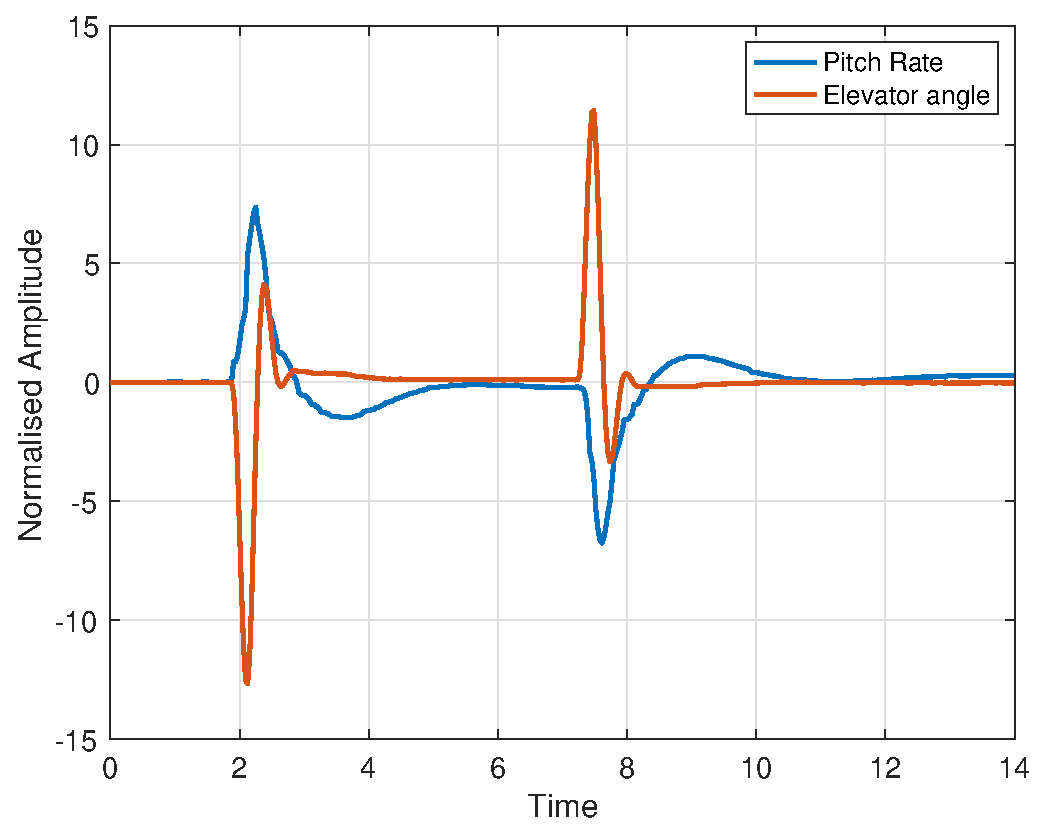
\includegraphics{EtoQ_IO.eps}
        \label{}
        \caption{}
    \end{figure}
    % The input & output
    % FFT + fit
    % Response + expected out (if exist)
    % root locus

% explanation on how it was made to work

\section{$\frac{N_z}{\delta_E}$ Elevator Deflection to Normal Acceleration at IRS}

\section{$\frac{r}{\delta_R}$ Rudder Deflection to Yaw Rate}

\section{$\frac{\phi}{\delta_A}$ Aileron Deflection to Roll Angle}

\end{document}